% This is samplepaper.tex, a sample chapter demonstrating the
% LLNCS macro package for Springer Computer Science proceedings;
% Version 2.20 of 2017/10/04
%
\documentclass[runningheads]{llncs}
%
\usepackage{graphicx}
% Used for displaying a sample figure. If possible, figure files should
% be included in EPS format.
%
% If you use the hyperref package, please uncomment the following line
% to display URLs in blue roman font according to Springer's eBook style:
% \renewcommand\UrlFont{\color{blue}\rmfamily}

\usepackage{fancyhdr} % Used for page numbers
\usepackage{float} % Lets you prevent LaTeX from repositioning images and tables using [H] specifier.

% Algorithms
\usepackage{algpseudocode}
\usepackage{algorithm}
\usepackage{amsmath}

% Tab
\usepackage{multirow}

\pagestyle{plain}
\fancyhf{} % Clear header and footer
\cfoot{\thepage} % Page number in the right footer

\begin{document}


%
\title{Efficient and secure implementation of AES-GCM in Jasmin - State of the art}


%
%\titlerunning{Abbreviated paper title}
% If the paper title is too long for the running head, you can set
% an abbreviated paper title here
%
\author{Noah Candaele\inst{1} \and Anthony Iozzia\inst{1} \and Sid Touati\inst{2} (supervisor) \and Benjamin Gregoire\inst{2} (co-supervisor) \and Jean-Christophe Léchenet\inst{2} (co-supervisor)}

%
\authorrunning{F. Author et al.}
% First names are abbreviated in the running head.
% If there are more than two authors, 'et al.' is used.
%
\institute{
Université Côte d'Azur, Sophia-Antipolis, France\\
\email{\{noah.candaele,anthony.iozzia\}@etu.univ-cotedazur.fr}
\and 
Inria research institute, Sophia-Antipolis, France\\
\email{\{sid.touati,benjamin.gregoire,jean-christophe.lechenet\}@inria.fr}
}



%
\maketitle              % typeset the header of the contribution
%

\thispagestyle{plain} % display page nb also on first page

%\begin{abstract}
%The abstract should briefly summarize the contents of the paper in
%15--250 words.
%
%\keywords{First keyword  \and Second keyword \and Another keyword.}
%\end{abstract}

%
%
%

\section{Introduction}

Cryptography, a specialized branch of mathematics and computer science, has distinct needs that differentiate it from general-purpose programming. Cryptographic programs require careful attention, such as focusing on certifying the code and ensuring stable performance to prevent security breaches. It's crucial to prioritize the strength and reliability of cryptographic implementations to protect sensitive information and prevent potential attacks.

Recognizing the distinctive nature of cryptographic applications, there has been a concerted effort in the development of programming languages specifically tailored to address the intricate demands of cryptography. These specialized languages aim to provide a secure and efficient environment for cryptographic operations, acknowledging the critical role they play in securing digital communication, financial transactions, and sensitive data.

This state of the art explores cryptographic programming languages, examining their unique features, design principles, and performance traits. It also explores advanced algorithms, specifically focusing on the widely used Advanced Encryption Standard (AES) and the authenticated encryption algorithm AES-GCM (Galois/Counter Mode). These algorithms are crucial components of cryptographic systems. We also underscore the potential for future implementation in Jasmin, a dedicated cryptographic language, highlighting the importance of such an implementation in advancing cryptographic functionality.

\section{Languages dedicated to cryptography}

\subsection{Some languages}
\subsubsection{HACL*:}
HACL*\cite{hacl_star_paper} (High-Assurance Cryptographic Library) is a programming language designed for writing high-assurance cryptographic code. It focuses on providing a formally verified and secure environment for cryptographic implementations, aiming to eliminate vulnerabilities and exploits in sensitive applications. One of its primary advantages is its emphasis on formal verification techniques, which enable mathematical proofs of code correctness, enhancing the overall security of cryptographic systems. HACL* supports a wide range of cryptographic primitives and is implemented in F*, a functional programming language that allows expressive specifications and formal reasoning. However, its disadvantages include a potentially steep learning curve due to the need for developers to understand formal methods and the limited scope of applications, as HACL* is specifically tailored for cryptographic tasks, making it less suitable for general-purpose programming. Additionally, the verification process can be resource-intensive, impacting development time.


\subsubsection{Qhasm:}
%Quantum High-Assurance Software Methodology
 Qhasm\cite{qhasm} is a project that aims to develop tools and interfaces for the high-speed generation of professional-quality software for various applications, particularly in the field of quantum computing.
However, it is important to note that Qhasm is in prototype form since 2007, and there are significant reasons for not using it in professional settings:
\begin{itemize}
    \item Tool Deficiencies: The existing Qhasm tools and interfaces, while capable of producing high-speed software, are not themselves of professional quality. They have many known deficiencies and areas that need improvement.
    \item Planned Rewrites: Each of the Qhasm tools has at least one complete rewrite planned, indicating ongoing development and potential instability in the current versions.
    \item Instability of .q language: The .q language used in Qhasm is not stable. If developers write code in .q files, they should anticipate extensive modifications for future Qhasm releases.
\end{itemize}


\subsubsection{Cryptol:} 
Cryptol\cite{cryptol} is a domain-specific language specifically designed for specifying and verifying cryptographic algorithms. It provides a concise and expressive syntax for describing cryptographic operations and protocols, allowing for formal verification and analysis of their security properties. 

One notable advantage of Cryptol is its ability to bridge the gap between high-level algorithmic descriptions and their low-level implementations, facilitating a more systematic and secure development process. Cryptol's type system aids in catching potential vulnerabilities early in the design phase, contributing to enhanced security. Additionally, Cryptol supports automated testing and formal verification, enabling developers to ensure the correctness and robustness of cryptographic code. 

However, challenges exist, such as a potential learning curve due to the specialized nature of the language. Integrating Cryptol into existing development workflows may require effort, and the ecosystem around Cryptol tools may not be as extensive as more widely adopted programming languages. Nonetheless, Cryptol stands out as a valuable tool for building and verifying secure cryptographic systems.

\subsection{Why we choose the Jasmin programming language}
Jasmin\cite{jasmin_paper}, as a verified programming language and compiler, stands out in the field of high performance and high-assurance cryptography. This platform offers a flexible programming environment that combines both high-level and low-level features. Programmers using Jasmin have the ability to optimize crucial aspects for performance, such as instruction selection and register allocation, while exploiting high-level concepts such as variables, functions, tables and loops to organize and check their code.

Jasmin benefits from a formal semantics that facilitates rigorous reasoning on the behavior of programs. This semantics is defined in Coq and can be used to directly interpret Jasmin programs.

The Jasmin compiler generates an efficient and predictable assembly code that preserves the properties of the source program.

The Jasmin workbench uses the EasyCrypt tool set for formal verification. Jasmin programs can be translated into corresponding EasyCrypt programs to prove functional correction, cryptographic security or security against auxiliary channel attacks (constant time).

Jasmin combines the best of all worlds: high-level language with high performance and high assurance. For these reasons, we will use Jasmin as the programming language for our implementations of cryptographic algorithms.



\section{Cryptography's Role in Digital Security}

The rapid evolution of Information and Communication Technology (ICT) has elevated the internet to a central platform for information in the 21st century. Despite this, ensuring the confidentiality, integrity, and availability of information transmitted over public networks remains a persistent challenge. Various methods, including information hiding through watermarking and steganography, as well as cryptographic techniques, have been extensively studied to enhance the security of data exchanged over unsecured networks.

Within the realm of cryptography, the primary objective is to safeguard information by rendering a secret message indecipherable to unauthorized parties, allowing only the sender and intended recipient to access its contents. This is achieved through the utilization of one or more secret keys. Cryptographic techniques can be broadly categorized as symmetric, where the same key is used for both encryption and decryption, or asymmetric, where distinct keys perform these functions.

Symmetric cryptographic techniques are particularly advantageous when securing substantial volumes of data. Indeed, asymmetric algorithms are more computationally intensive. Noteworthy examples of symmetric cryptographic algorithms include the Data Encryption Standard (DES), Triple DES, and the widely adopted Advanced Encryption Standard (AES). Among these, AES has emerged as the most prevalent and extensively utilized method for ensuring the security of sensitive information in the digital landscape.

\subsection{The Advanced Encryption Standard (AES)}

The Advanced Encryption Standard algorithm, established as the encryption standard for digital data by the US National Institute of Standards and Technology (NIST), is a symmetric key algorithm. Operating as an iterative round block cipher, it processes 128-bit plaintext using key lengths of 128, 192, and 256 bits. The chosen key length dictates the number of encryption and decryption rounds, 10, 12, and 14 rounds. It is generally understood that a larger key length enhances cryptographic strength. The AES algorithm, developed by a team led by Vincent Rijmen and Joan Daemen, consists of four invertible transformations: SubBytes, ShiftRows, MixColumns, and AddRoundKey.

Each of these transformations is applied in every encryption round, except for the last round, where the MixColumns transformation is deliberately excluded. This omission in the final round aims to maintain symmetry between the encryption and decryption processes. The transformations can be described as follows:

\begin{itemize}
    \item SubBytes Transformation: During this phase, each byte in the block is substituted with a corresponding byte from a fixed substitution table (S-box). This non-linear substitution, facilitated by the S-box, introduces intricacy to the algorithm, fortifying its resistance against cryptanalysis.
    \item ShiftRows Transformation: This operation entails shifting the rows of the block, contributing to diffusion and introducing complexity. The offset for each row's shift varies, enhancing the overall confusion in the encrypted data.
    \item MixColumns Transformation: In this step, a mathematical operation is applied to each column of the block. This operation fosters diffusion across columns, significantly contributing to the algorithm's resistance against linear attacks.
    \item AddRoundKey Transformation: The final step involves a bitwise XOR operation between a round key, generated from the original encryption key using a key schedule, and the state matrix. This step introduces the key into the encryption process, ensuring that each round employs a unique portion of the key, thereby boosting the overall security of the algorithm.
\end{itemize}

Collectively, these transformations establish a robust and secure encryption process. The deliberate symmetry in the final round ensures consistency between encryption and decryption procedures.

\subsection{Algorithme specification}



The input block, output block, and State of AES are all 128 bits. We define $N_b = 4$, which is the number of 32-bit words, or columns, in the State structure.

The Cipher Key ($K$) can have the lengths 128, 192, and 256 bits. These lengths are denoted by $N_k = 4, 6,$ or $8$, indicating the number of 32-bit words, or columns, that compose the Cipher Key.

The AES algorithm adapts to different key sizes, influencing the number of rounds ($N_r$) in its cryptographic process, which are defined as $N_r = 10$ for $N_k = 4$, $N_r = 12$ for $N_k = 6$, and $N_r = 14$ for $N_k = 8$.

The Key-Block-Round combinations are given in Fig. \ref{fig:table_key_block_round_combinations}. The AES encryption algorithm can be found in Algorithm \ref{fig:algo_aes_encrypt}. The AES decryption algorithm can be found in Algorithm \ref{fig:algo_aes_decrypt}.


\begin{figure}[ht]
    \centering
    \begin{tabular}{c|c|c|c|}
        \cline{2-4}
        & \textbf{\begin{tabular}[c]{@{}c@{}}Key Length\\ (Nk words)\end{tabular}} & \textbf{\begin{tabular}[c]{@{}c@{}}Block Size\\ (Nb words)\end{tabular}} & \textbf{\begin{tabular}[c]{@{}c@{}}Number of\\ Rounds\\ (Nr)\end{tabular}} \\ \hline
        \multicolumn{1}{|c|}{\textbf{AES-128}} & 4 & 4 & 10 \\ \hline
        \multicolumn{1}{|c|}{\textbf{AES-192}} & 6 & 4 & 12 \\ \hline
        \multicolumn{1}{|c|}{\textbf{AES-256}} & 8 & 4 & 14 \\ \hline
    \end{tabular}
    \caption{Key-Block-Round Combinations}
    \label{fig:table_key_block_round_combinations}
\end{figure}


\begin{algorithm}[hbt!]
\caption{Pseudocode for AES encryption. Src: NIST FIPS\cite{AES_NIST}}
\begin{algorithmic}[1] % [1] = line numbers
    \Procedure{AesEncrypt}{$\text{in}, \text{Nr}, \text{w}$}
        \State $\text{state} \gets \text{in}$
        \State $\text{state} \gets \Call{AddRoundKey}{\text{state}, \text{w}[0..3]}$
        \For{$\text{round}$ \textbf{from} $1$ \textbf{to} $\text{Nr} - 1$}
            \State $\text{state} \gets \Call{SubBytes}{\text{state}}$
            \State $\text{state} \gets \Call{ShiftRows}{\text{state}}$
            \State $\text{state} \gets \Call{MixColumns}{\text{state}}$
            \State $\text{state} \gets \Call{AddRoundKey}{\text{state}, \text{w}[4 \times \text{round}..4 \times \text{round} + 3]}$
        \EndFor
        \State $\text{state} \gets \Call{SubBytes}{\text{state}}$
        \State $\text{state} \gets \Call{ShiftRows}{\text{state}}$
        \State $\text{state} \gets \Call{AddRoundKey}{\text{state}, \text{w}[4 \times \text{Nr}..4 \times \text{Nr} + 3]}$
        \State \Return $\text{state}$
    \EndProcedure
\end{algorithmic}
\label{fig:algo_aes_encrypt}
\end{algorithm}

While AES encryption transforms plaintext into ciphertext through a series of substitution, permutation, and key addition steps, AES decryption reverses this process to recover the original plaintext.

\begin{algorithm}[hbt!]
\caption{Pseudocode for AES decryption. Src: NIST FIPS\cite{AES_NIST}}
\begin{algorithmic}[1] % [1] = line numbers
    \Procedure{AesDecrypt}{$\text{in}, \text{Nr}, \text{w}$}
        \State $\text{state} \gets \text{in}$
        \State $\text{state} \gets \Call{AddRoundKey}{\text{state}, \text{w}[4 \times \text{Nr}..4 \times \text{Nr} + 3]}$
        \For{$\text{round \textbf{from} Nr} - 1$ \textbf{downto} $1$}
            \State $\text{state} \gets \Call{InvShiftRows}{\text{state}}$
            \State $\text{state} \gets \Call{InvSubBytes}{\text{state}}$
            \State $\text{state} \gets \Call{AddRoundKey}{\text{state}, \text{w}[4 \times \text{round}..4 \times \text{round} + 3]}$
            \State $\text{state} \gets \Call{InvMixColumns}{\text{state}}$
        \EndFor
        \State $\text{state} \gets \Call{InvShiftRows}{\text{state}}$
        \State $\text{state} \gets \Call{InvSubBytes}{\text{state}}$
        \State $\text{state} \gets \Call{AddRoundKey}{\text{state}, \text{w}[0..3]}$
        \State \Return $\text{state}$
    \EndProcedure
\end{algorithmic}
\label{fig:algo_aes_decrypt}
\end{algorithm}


\newpage
\subsection{AES Galois Counter Mode (AES-GCM)}

AES-CBC (Cipher Block Chaining) is a mode of operation for the Advanced Encryption Standard (AES). In AES-CBC, each plaintext block is XORed with the previous ciphertext block before encryption. This chaining mechanism introduces dependencies between blocks, enhancing security by preventing identical plaintext blocks from producing identical ciphertext blocks.

\begin{figure}[ht] % ht = auto, H = fixed
    \centering
    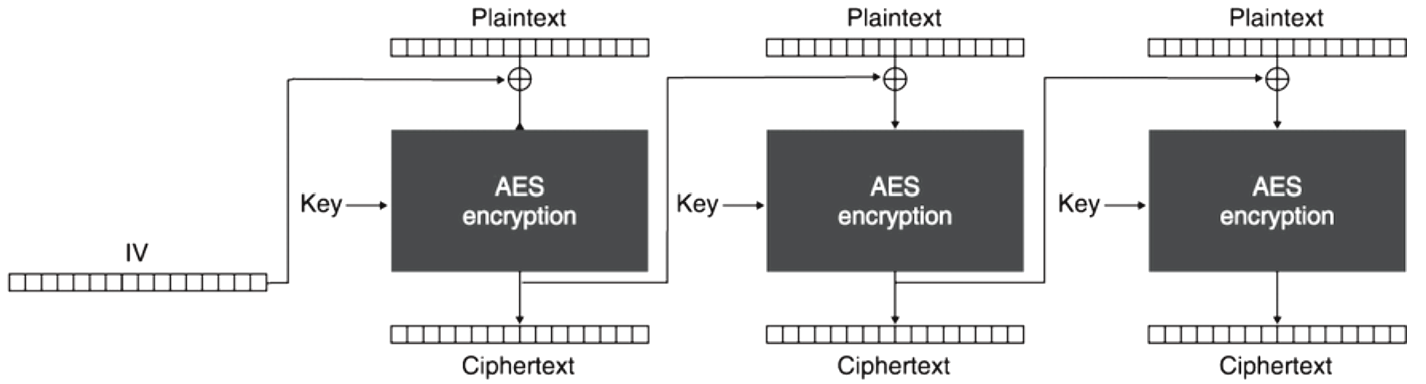
\includegraphics[scale=0.55]{resources/AES_CBC.png}
    \caption{The CBC mode of operation with AES. Src: \cite{book_real_world_crypto}}
\end{figure}

AES-GCM (Galois/Counter Mode) is another mode of operation for AES. Unlike AES-CBC, GCM combines encryption and authentication, providing both confidentiality and integrity. GCM operates by dividing the data into blocks, encrypting each block using AES in counter mode, and then incorporating an authentication tag. The tag is generated using Galois field multiplication, ensuring data integrity. AES-GCM is widely used in secure communications, such as in TLS (Transport Layer Security) for securing internet connections. It offers efficient and robust protection against both eavesdropping and tampering.

\begin{figure}[ht] % ht = auto, H = fixed
    \centering
    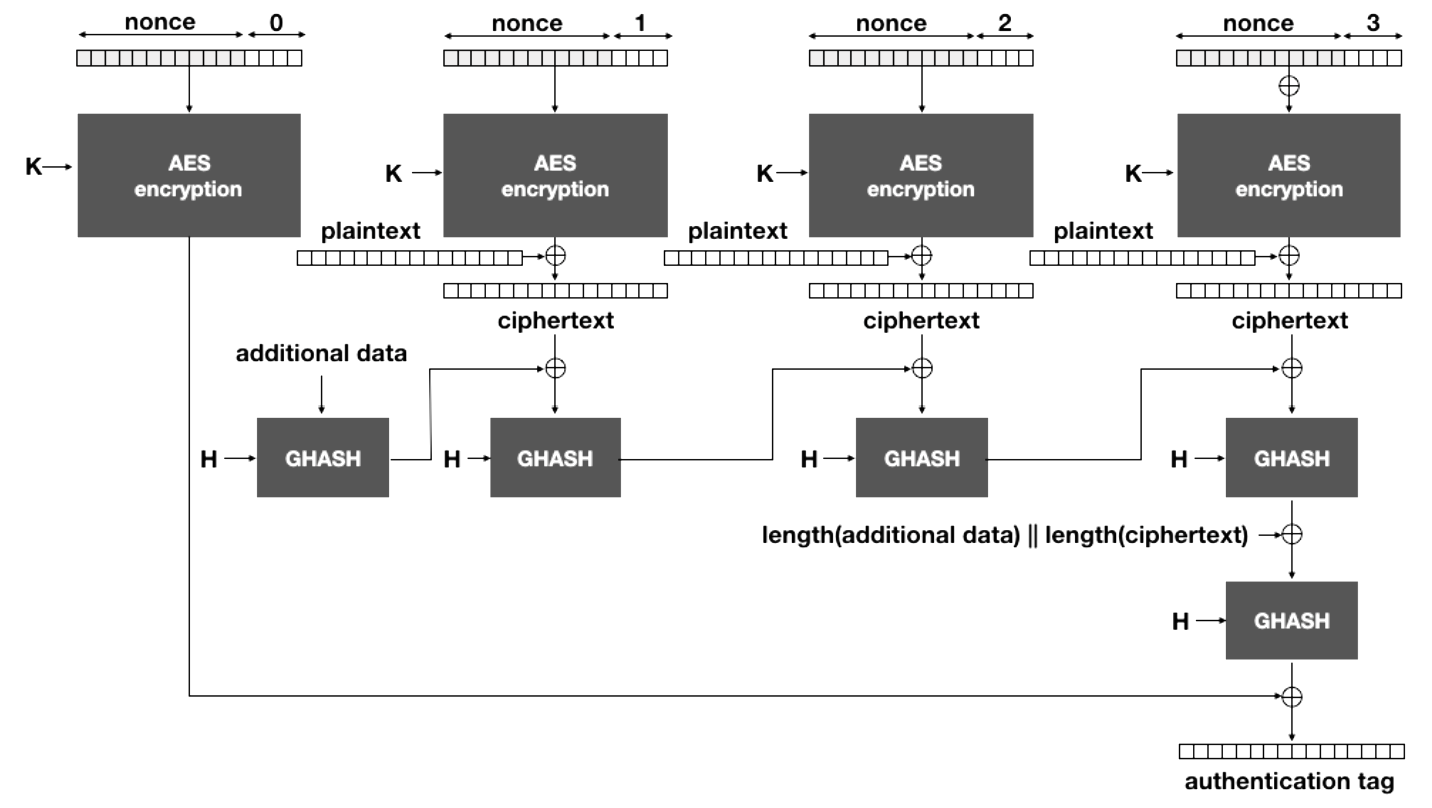
\includegraphics[scale=0.55]{resources/AES_GCM.png}
    \caption{The AES GCM encryption process. Src: \cite{book_real_world_crypto}}
\end{figure}

\section{Attacks on high-assurance cryptographic code}

Vulnerabilities can lead to severe consequences, especially for cryptographic code, where the stakes are exceptionally high. High-assurance code undergoes rigorous formal verification processes and adheres to strict development standards, significantly reducing the likelihood of common vulnerabilities. However, potential threats persist, as we will discuss in this section.


\subsection{Side-Channel Attacks}
Side-channel attacks\cite{paper_side_channel_attacks} exploit information leaked during the execution of cryptographic algorithms.

\subsubsection{Timing attacks}
Timing attacks are a type of side-channel attack that exploits variations in the time taken for specific operations. By carefully measuring the time it takes for a system to perform certain computations, an attacker can gain insights into sensitive information, such as cryptographic keys. The variations in execution time may reveal patterns that allow the attacker to infer details about the underlying data or algorithms.

For example, consider an application that performs user authentication by comparing a hashed user-entered password with the stored hashed password. If the system takes less time to respond when the first character of the password is correct, an attacker could iteratively guess each character and measure the response time. The correct character will result in a slightly longer response time due to the additional computation, allowing the attacker to deduce the correct password one character at a time.

To mitigate timing attacks, algorithms must have constant execution time regardless of input.

\subsubsection{Cache attacks}
Cache attacks are a class of side-channel attacks that exploit variations in cache access times to extract sensitive information. By observing the time it takes to access specific memory locations, an attacker can infer patterns of memory usage, potentially revealing details about confidential data like cryptographic keys. Cache attacks often target the shared cache in multi-core processors, where one core's activities can impact the cache behavior seen by another core.

For example, in a Prime+Probe Attack, an attacker ``primes'' the cache by loading data into it, then measures the time it takes to ``probe'' the cache by accessing certain memory locations. If the target system is performing cryptographic operations, the attacker can correlate the timing information with specific operations, allowing them to deduce sensitive information like cryptographic keys.

Mitigating cache attacks involves using cache-timing-resistant algorithms and implementing secure coding practices. We should aim to minimize observable variations in cache behavior during cryptographic operations. Techniques such as data obfuscation, padding, or algorithmic modifications can be employed to make the access patterns less predictable. Additionally, ensuring that sensitive data is not shared in the same cache line with non-sensitive data can help reduce the risk of cache-based side-channel attacks.

\subsubsection{Power Analysis Attacks}
Power analysis attacks are another subset of side-channel attacks that exploit variations in power consumption during the execution of cryptographic algorithms. By analyzing the power consumption patterns of a device, an attacker can infer information about the internal computations, potentially revealing cryptographic keys or other sensitive data.

There are two primary types of power analysis attacks:

\begin{enumerate}
    \item \textbf{Simple Power Analysis (SPA):} SPA involves analyzing the power consumption of a device over time to identify patterns associated with specific operations. For instance, cryptographic algorithms often involve modular exponentiation, and the power consumption during this operation may exhibit recognizable patterns. Once identified, these patterns can be correlated to extract information about the cryptographic key.
    \item \textbf{Differential Power Analysis (DPA):} DPA is a more sophisticated attack that involves statistical analysis of power consumption differences between different inputs or operations. By observing the power variations, an attacker can notice patterns related to the data being processed. This allows them to deduce information about secret keys or plaintext data.

\end{enumerate}

To counter power analysis attacks, cryptographic implementations can include techniques like constant-time algorithms, which ensure that the power consumption remains constant regardless of the processed data.


\subsection{Mitigating High-Assurance Cryptographic Code Vulnerabilities}
Understanding and mitigating these side-channel vulnerabilities is crucial for developing secure cryptographic code. The most important mitigation that we can implement is ensuring that our algorithms have constant execution time, regardless of input.


\section{Conclusion}

In conclusion, the field of high-assurance cryptographic code is essential for ensuring the security of sensitive information. Specialized cryptographic programming languages like Jasmin provide a robust platform for developing secure and efficient cryptographic implementations. The Advanced Encryption Standard (AES) and its mode of operation, AES-GCM, play a central role in cryptographic systems, providing confidentiality and integrity.

However, the challenges of side-channel attacks, such as timing attacks, cache attacks, and power analysis attacks, pose potential threats to high-assurance cryptographic code. Mitigating these vulnerabilities requires constant-time algorithms, secure coding practices, and careful consideration of potential information leaks during execution.

In this state of the art, we explored various cryptographic programming languages, focusing on Jasmin due to its unique combination of high-level and low-level features. We delved into the specifications of the AES algorithm and its widely used mode, AES-GCM. Additionally, we discussed potential attacks on high-assurance cryptographic code and highlighted mitigation strategies.

As the digital landscape continues to evolve, the importance of high-assurance cryptographic code remains paramount. Ongoing research and development in this field, coupled with rigorous verification processes, will contribute to the ongoing effort to secure digital communication and protect sensitive information from potential threats.



% ---- Bibliography ----
%
% BibTeX users should specify bibliography style 'splncs04'.
% References will then be sorted and formatted in the correct style.
%
% \bibliographystyle{splncs04}
% \bibliography{mybibliography}
%
\newpage
\begin{thebibliography}{8}

\bibitem{hacl_star_paper}
Jean Karim Zinzindohouee, Karthikeyan Bhargavan, Jonathan Protzenko and Benjamin Beurdouche: HACL* A Verified Modern Cryptographic Library, Cryptology ePrint Archive, 2017 \url{https://ia.cr/2017/536}

\bibitem{qhasm}
Qhasm*, \url{https://cryptojedi.org/programming/index.shtml}. Last accessed 26 Jan 2024

\bibitem{cryptol}
Cryptol: The language of Cryptography \url{https://cryptol.net/files/ProgrammingCryptol.pdf}.

\bibitem{modified_AES}
Abikoye, Oluwakemi Christiana and Haruna, Ahmad Dokoro and Abubakar, Abdullahi and Akande, Noah Oluwatobi and Asani, Emmanuel Oluwatobi: Modified Advanced Encryption Standard Algorithm for Information Security. Symmetry 2019 \doi{10.3390/sym11121484}

\bibitem{book_real_world_crypto}
David Wong.: Book: Real-World Cryptography. Manning,(2021)

\bibitem{jasmin_paper}
Almeida, Jos{\'e} Bacelar and Barbosa, Manuel and Barthe, Gilles and Blot, Arthur and Gr{\'e}goire, Benjamin and Laporte, Vincent and Oliveira, Tiago and Pacheco, Hugo and Schmidt, Benedikt and Strub, Pierre-Yves, Jasmin: High-Assurance and High-Speed Cryptography, CCS 2017 - Proceedings of the 2017 ACM SIGSAC Conference on Computer and Communications Security, Oct 2017, Dallas \url{https://hal.science/hal-01649140}.

\bibitem{vale_paper}
Bond, Barry and Hawblitzel, Chris and Kapritsos, Manos and Leino, K. Rustan M. and Lorch, Jacob R. and Parno, Bryan and Rane, Ashay and Setty, Srinath and Thompson, Laure, Vale: Verifying High-Performance Cryptographic Assembly Code, USENIX Association 2017 \url{https://dl.acm.org/doi/10.5555/3241189.3241261}.

\bibitem{paper_side_channel_attacks}
Antoine Geimer, Mathéo Vergnolle, Frédéric Recoules, Lesly-Ann Daniel, Sébastien Bardin, Clémentine Maurice: A Systematic Evaluation of Automated Tools for Side-Channel Vulnerabilities Detection in Cryptographic Libraries. arXiv e-prints 2023 \doi{10.48550/arXiv.2310.08153}

\bibitem{AES_NIST}
Morris Dworkin and Elaine Barker and James Nechvatal and James Foti and Lawrence Bassham and E. Roback and James Dray: Advanced Encryption Standard (AES). NIST FIPS 2001 updated 2023 \doi{10.6028/NIST.FIPS.197-upd1}

%%%%%%%%%% Formats examples
%\bibitem{ref_article1}
%Author, F.: Article title. Journal \textbf{2}(5), 99--110 (2016)

%\bibitem{ref_lncs1}
%Author, F., Author, S.: Title of a proceedings paper. In: Editor,
%F., Editor, S. (eds.) CONFERENCE 2016, LNCS, vol. 9999, pp. 1--13.
%Springer, Heidelberg (2016). \doi{10.10007/1234567890}

%\bibitem{ref_book1}
%Author, F., Author, S., Author, T.: Book title. 2nd edn. Publisher,
%Location (1999)

%\bibitem{ref_proc1}
%Author, A.-B.: Contribution title. In: 9th International Proceedings
%on Proceedings, pp. 1--2. Publisher, Location (2010)

%\bibitem{ref_url1}
%LNCS Homepage, \url{http://www.springer.com/lncs}. Last accessed 4
%Oct 2017
%%%%%%%%%%%

\end{thebibliography}


%\begin{figure}[ht] % ht = auto, H = fixed
%    \centering
%    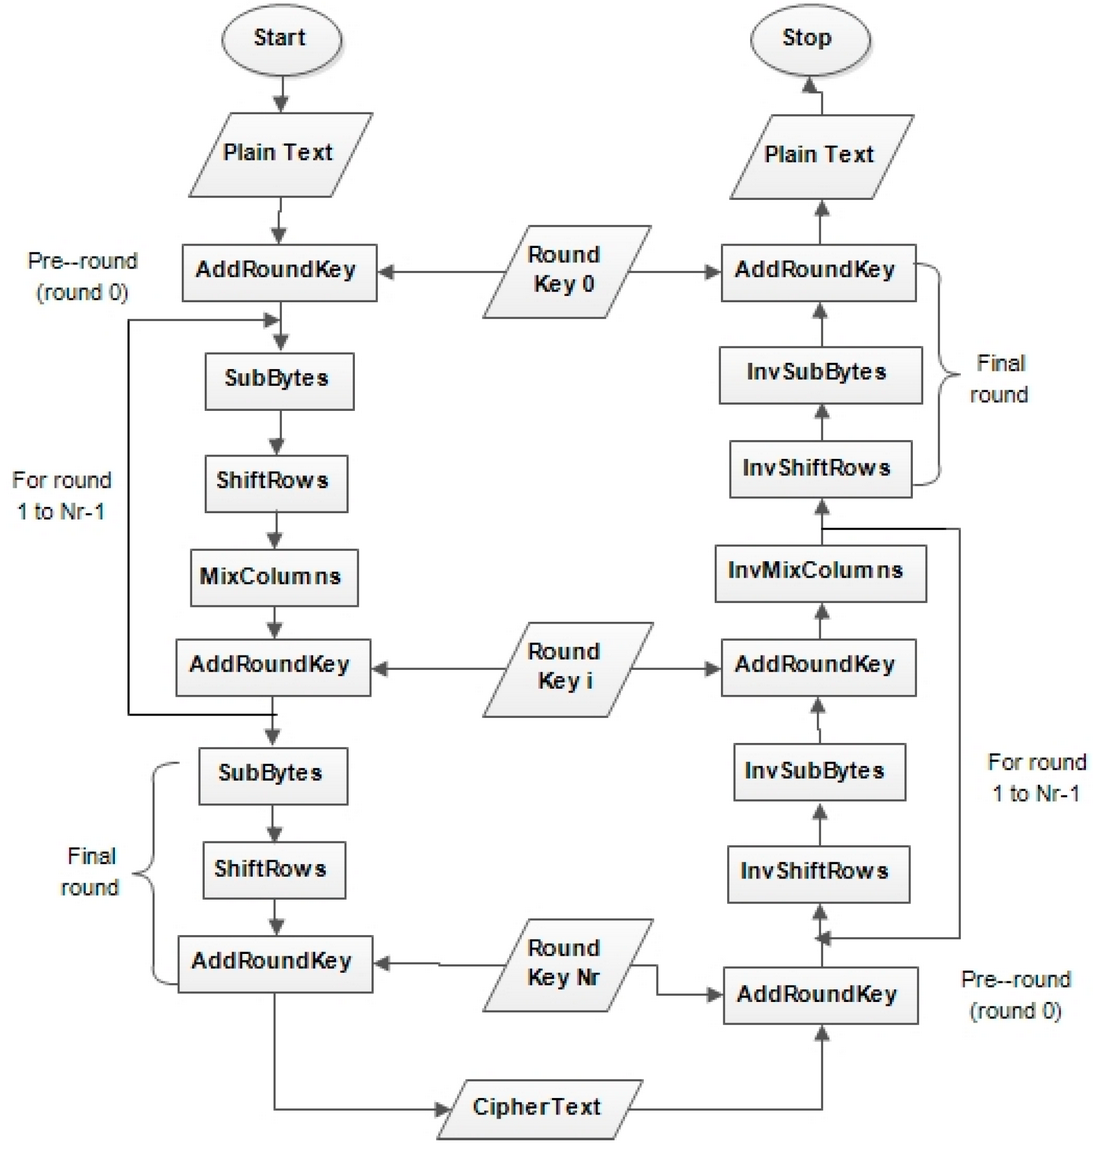
\includegraphics[scale=0.70]{resources/AES_schema.png}
%    \caption{Structure of the Advanced Encryption Standard (AES) %Algorithm. Src: \cite{modified_AES}}
%\end{figure}

\newpage
\appendix
\section{Appendix: Full-time period progress plan}

In this appendix, we outline the tasks planned for the full-time period.

\subsection{Implementation of AES in Jasmin}
The first part consists in implementing the standard version of AES in Jasmin. We will do it in two parts:
\begin{itemize}
    \item An initial version using tables. This version may not have constant-time execution regardless of the input.
    \item A final version using 128-bit AES-NI (Advanced Encryption Standard New Instructions), which is a hardware accelerated version of AES.
\end{itemize}

\subsection{Implementation of AES-GCM in Jasmin}
The second part consists in implementing the Galois/Counter Mode of AES (AES-GCM). There will be two parts:
\begin{itemize}
    \item The main version, implementing AES-GCM in regular Jasmin.
    \item A prototype version, using invented instructions for code clarity. We will then provide a documented list of these invented instructions to Jasmin developers.
\end{itemize}

\end{document}
